\documentclass[a4paper,kulak]{kulakarticle}

\usepackage[utf8]{inputenc}
\usepackage[dutch]{babel}
\usepackage[]{amsmath}
\usepackage{float}
\usepackage{subcaption}
\usepackage{graphicx,wrapfig,lipsum}

\date{Academiejaar 2018-2019}
\address{
  Informatica \\
  Statistische modellen en data-analyse \\
  Prof. Stefan Van Aelst \& Stijn Rebry}
\title{Verslag project 1}
\author{Thomas Bamelis R0640219 \& Michiel Jonckheere R0665594}

\begin{document}

\maketitle

\tableofcontents
\newpage
\section*{Introductie}
In dit verslag wordt nagegaan hoe de oorzaken van overlijden verschillen tussen landen en regio's in
de wereld. Er zijn schattingen van het aantal overlijdens beschikbaar voor 183 landen,
opgesplitst naar 32 verschillende doodsoorzaken. De landen worden gegroepeerd in 6 groepen volgens
geografische ligging en 2 groepen naargelang de globale ontwikkeling van het betreffende land. De gegevens
met betrekking tot de doodsoorzaken zijn afkomstig van de Wereldgezondheidsorganisatie \cite{ghe} en betreffen
het jaar 2016, de indeling in groepen is deze volgens de Verenigde Naties \cite{vn}. 
Deze gegevens werden verwerkt en geïnterpreteerd als proporties van de soorten sterfgevallen per land.

\section{Clustering}
Als eerste werd een cluster-analyse uitgevoerd op de gegevens. Eerst bespreken we de gegevens zonder schalen, daarna met.
\subsection{Zonder schalen}
Om een idee te krijgen van hoeveel clusters er best worden genomen, werden het agglomerate nesting algoritme en divisive analysis toegepast.
Agglomerate nesting werd gedaan met de volgende dissimilariteiten: group average, nearest neighbour en furthest neighbour, in die volgorde met daarna divisive analysis.
Zie figuren \ref{fig:hcnd} en \ref{fig:hcnb} in de bijlage \ref{b}.
Gegeven deze figuren lijkt het meest aannemelijk om 2, 4 en 6 klassen te proberen.
De gebruikte clustering algoritmes zijn in volgorde k-means, partitioning around mediods en fuzzy analysis.
De clustering ermee voor 2, 4 en 6 klassen werd geëvalueerd via een silhouette plot en een clusplot.
Zie figuur \ref{fig:cne}.
Hieruit blijkt dat partitioning around mediods met 2 clusters het beste presteert met een silhouette coëfficiënt van 0.50 (cluster 1 : 0.69 en cluster 2 : 0.43).
Dit is niet bepaald goed en balanceert op het randje van een zwakke structuur.
\subsection{Met schalen}
 We trekken hierbij dezelfde conclusies omtrent het aantal klassen, 2, 4, en 6.
 Zie figuren \ref{fig:hcd} en \ref{fig:hcb}.
 Na dezelfde clustering algoritmes toegepast te hebben (figuur \ref{fig:ce}), is de best geobserveerde silhouette coëfficiënt 0.23.
 Hieruit besluiten we dat clustering met schalen aanzienlijk slechter is dan zonder schalen.
 We besluiten dus verder te werken met het beste resultaat zonder schalen.
\subsection{Beschrijving clusters}
We bekijken nu nader de twee clusters geselecteerd door pam met twee clusters zonder schalen.
We bekijken eerst hoeveel landen uit een bepaalde regio in een bepaalde cluster zitten.
\begin{table}[ht]
\centering
\begin{tabular}{rrrrrr}
  \hline
 Cluster & Africa & America & Asia & Europe & Oceania \\ 
  \hline
1 &  45 &   0 &   2 &   0 &   1 \\ 
  2 &   9 &  33 &  44 &  40 &   9 \\ 
   \hline
\end{tabular}
\end{table}

Hieruit kunnen we afleiden dat 45 van de 48 landen in de eerste cluster Afrikaanse landen zijn.
Cluster twee bevat bijna alle landen uit America, Asia, Europe en Oceania.
Ze bevat ook nog 9 Afrikaanse landen.
De eerste cluster neem dus 4/5 van de Afrikaanse landen en op 3 landen na.
Het clustering algoritme vindt dus vooral onderscheid tussen Afrikaanse landen tegenover de rest van de wereld qua doodsoorzaken.

\begin{table}[ht]
\centering
\begin{tabular}{rrrrr}
  \hline
 Cluster & \#N/B & Developed & Developing & Transition \\
  \hline
1 &   1 &   0 &  47 &   0 \\
  2 &   0 &  36 &  90 &   9 \\
   \hline
\end{tabular}
\end{table}

Clustering tegenover ontwikkeling toont dat de eerste cluster enkel developing landen selecteert, op Congo na waarvan de ontwikkeling onbepaald is.
Het valt echter op dat cluster twee dubbel zoveel developing landen selecteert vergeleken met de eerste cluster, maar ook alle developed en transition landen.
Het is dus niet zo dat de eerste cluster focused op alle developing landen.
Als we dit samen leggen met de region table, kunnen we besluiten dat de eerste cluster hoofdzakelijk Afrikaanse developing landen bevat en de tweede cluster ``de rest''. \newline
Daarnaast kunnen we de verschillen van tussen de clusters bekijken qua doodsoorzaken.
We plotten daarom de marginale gemiddelden van de eerste cluster, afgetrokken met de marginale gemiddelden van de tweede cluster.
Zie figuur \ref{fig:dm}.
Als we de drie hoofdcategoriën van doodsoorzaken bekijken (de verschillende kleuren), blijkt dat communicable, maternal, perinatal and nutritional conditions meer voorkomen bij de eerste cluster dan bij de tweede.
We zien ook dat twee noncommunicable diseases aanzienlijk meer voorkomen in de tweede cluster, met nog eens 5 van die doodsoorzaken licht meer voorkomen in de tweede cluster.
Over de injuries tussen de twee clusters valt niets significants te zeggen. \newline
Met dit alles samen kunnen we besluiten dat de meeste Afrikaanse landen die developing zijn een proportioneel opvallend hoger aantal  communicable, maternal, perinatal and nutritional conditions bevatten en een proportioneel lager aantal noncommunicable diseases hebben tegenover de rest van de wereld.



\section{Principaalcomponentenanalyse}
%todo herschrijven, enkel naar geschaalde data kijken

Voor de principaalcomponentenanalyse wordt enkel gekeken naar de geschaalde gegevens. De eerste vier principaalcomponenten verklaren ongeveer 52\% van de variantie van de geschaalde data. Vanaf de vijfde principaalcomponent zijn de verschillen van de cumulatieve proporties van de variantie tussen de opeenvolgende principaalcomponenten kleiner. Dit is ook te zien in tabel \ref{table:pca} Daarom gaan we hier verder met enkel de vier eerste principaal componenten.

\begin{table}[ht]
	\centering
	\begin{tabular}{cccccc}
		\hline 
		PC1 & PC2 & PC3 & PC4 & PC5 & PC6 \\ 
		29.7\% & 40.4\% & 46.5\% & 52.3\% & 56.5\% & 60.4\%\\ 
		\hline 
	\end{tabular} 
	\caption{De cumulatieve proportie van de variantie van de eerste zes principaalcomponenten van de geschaalde data.}
	\label{table:pca}
\end{table}


\subsection{PC1}
Voor de \textit{Communicable, maternal, perinatal and nutritional conditions}, de meeste \textit{Unintentional Injuries}, \textit{Congenital Anomalies} en \textit{Sudden Infant Death Syndrome} vinden we de meest negatieve waarden tussen -0.2 en -0.3. De grootste positieve waarden vinden we voor de variabelen \textit{Malignant Neoplasms} en \textit{Cardiovascular Diseases} vinden we hoge positieve waarden, respectievelijk 0.28 en 0.23. Bij hogere PC1 waarden zullen er meer doden vallen door \textit{Malignant Neoplasms} en \textit{Cardiovascular Diseases}.

Als we dit bekijken voor de landen dan vinden we dat alle Europese landen de meest positieve PC1 waarden hebben en de meeste Afrikaanse landen de meest negatieve PC1 waarden. Dit is te zien in figuur \ref{fig:vglPC}. Uit deze figuur kunnen we ook afleiden dat Amerikaanse landen voornamelijk een positieve PC1 waarde hebben. Voor de volgende besprekingen van PC2, PC3 en PC4 kan figuur \ref{fig:vglPC} ook steeds worden gebruikt ter verduidelijking. We kunnen besluiten dat landen met een sterk negatieve PC1 waarde uit de regio Afrika komen. Bij een sterk positieve PC1 waarde is de kans het grootst dat het land in Europa gelegen is. 

Bij het kijken naar de ontwikkeling, zien we dat de ontwikkelingslanden overal verspreid zitten. De overgangs- en ontwikkelde landen hebben een grote positieve waarde. Dit hangt natuurlijk ook samen met het feit dat de meeste overgangs- en ontwikkelde landen in Europa liggen. We kunnen hier een vrij gelijkaardig besluit trekken als hierboven namelijk: bij een sterk negatieve PC1 waarde zal het land een ontwikkelingsland zijn en bij een sterk positieve PC1 waarde zal het land waarschijnlijk een ontwikkeld of overgangsland zijn.



\subsection{PC2}
De meest positieve waarden voor PC2 zijn voor de variabelen \textit{Diabetes Mellitus} en \textit{Cardiovascular Diseases}, met de respectievelijke waarden 0.16 en 0.18. Voor de variabelen \textit{Other Neoplasms}, \textit{Musculoskeletal Diseases}, \textit{Falls} en \textit{Other Unintentional Injuries} vinden we de meest negatieve PC2 waarden. Deze waarden zijn respectievelijk -0.31, -0.37, -0.29 en -0.31. 

De PC2 waarden per regio zijn redelijk verspreid en is er niet direct een conclusie uit te trekken dat in de ene regio opmerkelijk veel landen met hoge of lage PC2 waarden zijn. De enige bemerking die hier kan gemaakt worden is dat Amerikaanse en Europese landen vooral negatieve PC2 waarden hebben. Landen uit Oceani\"e hebben posieve PC2 waarden. 

Bij ontwikkeling is vooral te zien dat de overgangslanden positieve PC2 waarden hebben en de ontwikkelde landen voornamelijk negatieve PC2 waarden. De waarden van de ontwikkelingslanden liggen nogal verspreid.






\subsection{PC3}
Voor de derde principaalcomponent zijn de grootste waarden 0.31 en 0.34 voor de variabelen \textit{Mental and Substance Use Disorder} en \textit{Self Harm}. Deze twee variabele zijn wel met elkaar in verband te brengen aangezien de doodsoorzaak \textit{Self Harm} vaak gepaard zal gaan met psychische stoornissen en verslavingen. De meest negatieve PC3 waarde is van de variabele \textit{Endocrine Blood Immune Disorder} met als waarde -0.30.

Bij deze principaalcomponent is het enkel opvallend dat alle landen uit Oceani\"e een negatieve PC3 waarde hebben. Bij Aziatische landen komen voornamelijk positieve waarden voor, ook de meest positieve waarden komen van landen uit Azi\"e. Landen uit de andere regio's hebben PC3 waarden die zowel positief als negatief zijn. 


Overgangslanden hebben hier hoge PC3 waarden, over de andere ontwikkelingen van landen valt er verder niets te vertellen.


\subsection{PC4}
De vierde principaalcomponent vergelijkt de variabele \textit{Interpersonal Violence} met \textit{Neurological Conditions} en \textit{Falls}. De PC4 waarden van deze drie variabelen zijn respectievelijk -0.48, 0.22 en 0.26. Hoe hoger de PC4 waarde, hoe minder \textit{Interpersonal Violence} er is in dat land. 


De meeste Europese en Afrikaanse landen hebben een positieve PC4 waarde en de meeste Amerikaanse landen hebben een negatieve PC4 waarde. 

Ontwikkelde en overgangslanden hebben bijna allemaal een positieve PC4 waarde. Er is 1 ontwikkeld land die geen positieve PC4 waarde heeft en dat is Isra\"el. Dit is te verklaren omdat Isra\"el een geweldadiger land is dan de rest van de ontwikkelde landen. 



\section{Multivariate Normaliteit}
Om de multivariate normaliteit van de data na te gaan moeten we eerst en vooral kijken of alle variabelen wel univariaat normaal verdeeld zijn. De univariate testen tonen aan dat alle variabelen niet univariaat normaal verdeeld zijn. Hierdoor kan de data ook geen multivariate normaliteit hebben. Ook na het toepassen van de \textit{logit} transformatie was geen enkele variabele normaal verdeeld. 

We kunnen hieruit dus besluiten dat de gegevens niet multivariaat normaal verdeeld zijn en we in de volgende sectie over classificatie geen methodes moeten toepassen waarvoor deze eigenschap vereist is. Het zal dus nutteloos zijn van naar de a posteriori-kansen te kijken. 


\section{Classificatie}
Bij de classificatie gaan we na in hoeverre het mogelijk is om de regio en ontwikkeling van een land te identificeren a.d.h.v. de doodsoorzaken. Er wordt gebruik gemaakt van de lineaire discriminantmethode en \textit{k-nearest neighbours} methode. Het was niet mogelijk van de kwadratische discriminantmethode toe te passen op de data omdat sommige groepen te klein zijn en er niet genoeg data over is.

\subsection{Regio} %TODO percentages bij lda en knn bijzetten ter verduidelijking
Om classificatie toe te passen op de regio van landen, zien we dat bij elke methode de \textit{actual error rate} vrij groot is (tussen de 25\% en 30\%). Dit betekent dat het moeilijk is om effectief de regio te bepalen van een land als de doodsoorzaken gegeven zijn. 46 van de 183 landen worden verkeerd ingedeeld bij de lineaire discriminantmethode. Als we dan kijken naar de \textit{k-nearest neighbours} methode, dan zien we dat deze \textit{AER} (30\%) iets groter is dan bij de LDA (25\%). Er werd gekeken naar \textit{k} = $\{2,3,4,5\}$. De beste methode voor het classificeren volgens de regio's is de lineaire discriminantmethode. 

Het is opmerkelijk dat alle Europese landen juist ingedeeld worden als een Europees land. Er zijn wel relatief veel landen uit andere regio's die ook als Europees land worden ingedeeld. 

\subsection{Ontwikkeling}
Om de ontwikkeling van de landen na te gaan met behulp van de doodsoorzaken, verkregen we betere error ratio's. Deze lagen allemaal dicht bij elkaar rond de 12\%. De beste \textit{AER} verkregen we bij de \textit{8-nearest neighbours} methode. Hierbij werden 21 van de 183 landen verkeerd ingedeeld volgens hun ontwikkeling. Deze landen komen voornamelijk uit Europa, Azi\"e en Amerika. De meeste landen die verkeerd ingedeeld worden zijn ontwikkelingslanden of overgangslanden en worden als ontwikkeld land geclassificeerd. Ontwikkelde landen die verkeerd zijn ingedeeld worden als een overgangsland ingedeeld. 

In de data zit er \'e\'en speciaal land (Congo) waarvan de ontwikkeling niet gekend is. Dit land wordt ingedeeld als een ontwikkelingsland. Aangezien Congo in Afrika ligt en we uit de gegeven data konden opmerken dat alle landen uit Afrika ontwikkelingslanden zijn, kunnen we hier wel concluderen dat Congo een ontwikkelingsland is. 

\section*{Besluit}

Omdat clustering en pca opvallend beter werken voor Afrikaanse landen, kunnen we besluiten dat Afrika in doodsoorzaken relatief veel verschilt tegenover de andere regio's.
Meer bepaald sterven opvallend meer mensen in Afrika aan overdraagbare ziektes en minder aan niet-overdraagbare ziektes dan in de rest van de wereld. 
Ook werkte pca en classificatie beter voor Europa.
De analyse voor de andere regio's verliep moeilijker.
De andere regio's verschilden intern sterk qua ontwikkeling, terwijl Afrika en Europa nagenoeg allemaal developing of developed landen zijn.
Dit zou kunnen verklaren waardoor deze analyse beter werkte voor Afrika en Europa.
Het R script produceert nog meer figuren die niet zijn meegeleverd in dit verslag die onze conclusies ondersteunen.

\begin{thebibliography}{9}
	
	\bibitem{ghe}
	Global Health Estimates 2016: Deaths by Cause, Age, Sex, by Country and by Region, 2000-2016.
	Geneva, World Health Organization; 2018.
	
	\bibitem{vn}
	Country classification, june 2018. Geneva, United Nations Conference on Trade and Development;
	2018.
	
\end{thebibliography}

\newpage
\section{Bijlage} \label{b}
\subsection{Clustering}
\subsubsection{Zonder schalen}
\begin{figure}[H]
	\centering
	\includegraphics[height=\textheight]{figures/hierachicalClusteringNoScalingDendogram.jpg}
	\caption{Hierchical clustering dendograms}
	\label{fig:hcnd}
\end{figure}
\begin{figure}[H]
	\centering
	\includegraphics[height=\textheight]{figures/hierachicalClusteringNoScalingBanner.jpg}
	\caption{Hierchical clustering bannerplots}
	\label{fig:hcnb}
\end{figure}
\begin{figure}[H]
	\centering
	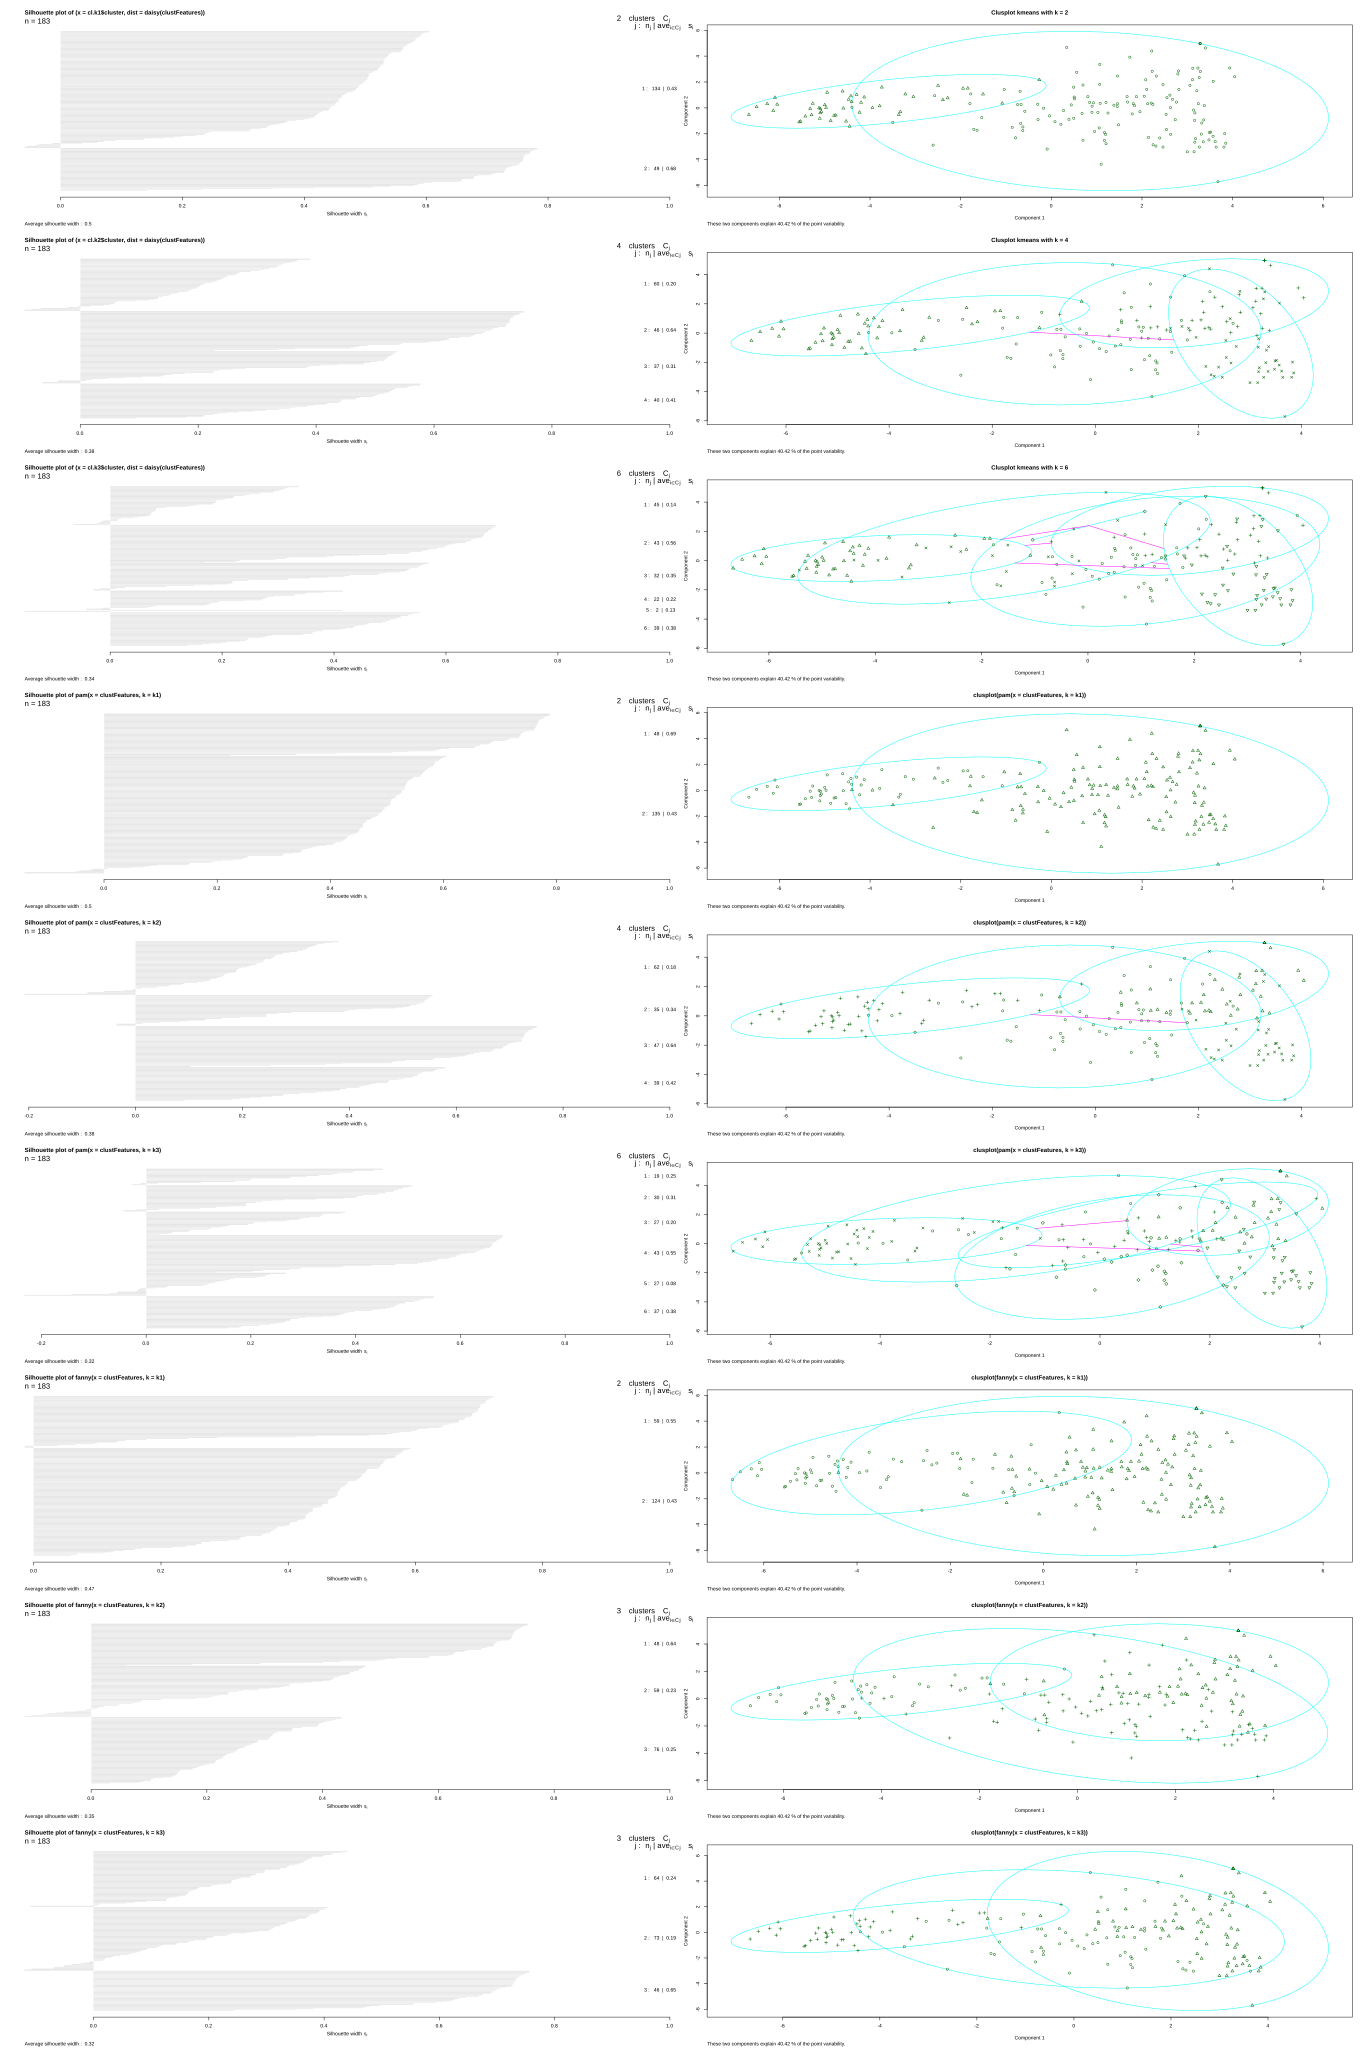
\includegraphics[height=\textheight]{figures/clusteringEvaluationNoScaling.jpg}
	\caption{Clustering evaluatie}
	\label{fig:cne}
\end{figure}
\subsubsection{Met schalen}
\begin{figure}[H]
	\centering
	\includegraphics[height=\textheight]{figures/hierachicalClusteringScaledDendogram.jpg}
	\caption{Hierchical clustering dendograms met schalen}
	\label{fig:hcd}
\end{figure}
\begin{figure}[H]
	\centering
	\includegraphics[height=\textheight]{figures/hierachicalClusteringScaledBanner.jpg}
	\caption{Hierchical clustering bannerplots met schalen}
	\label{fig:hcb}
\end{figure}
\begin{figure}[H]
	\centering
	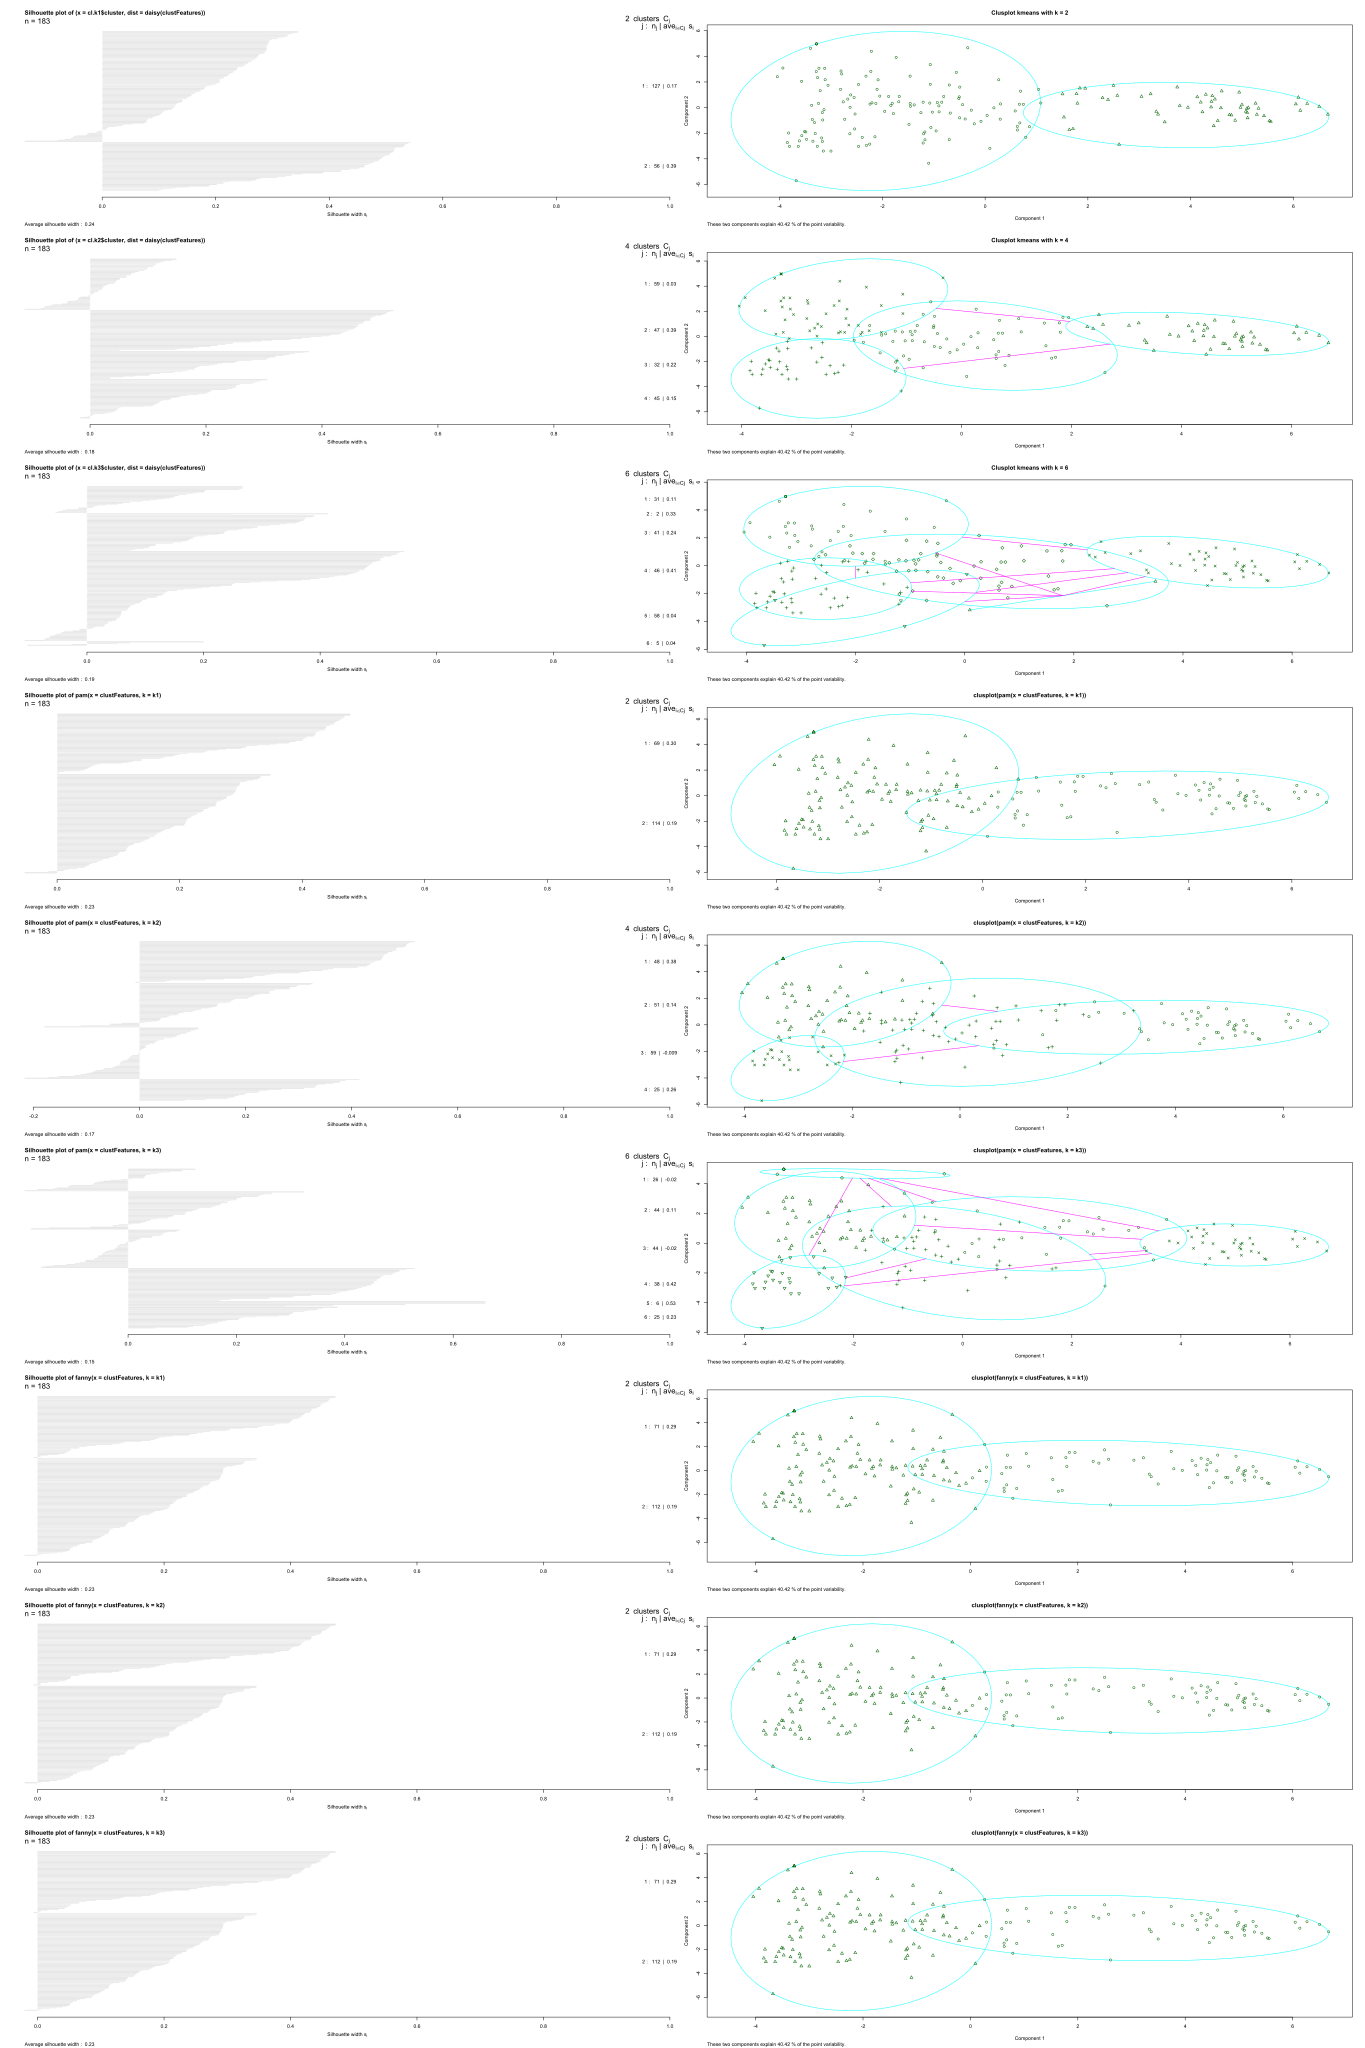
\includegraphics[height=\textheight]{figures/clusteringEvaluationScaled.jpg}
	\caption{Clustering evaluatie met schalen}
	\label{fig:ce}
\end{figure}

 \subsection{Beschrijving clusters}

\begin{figure}[H]
	\centering
	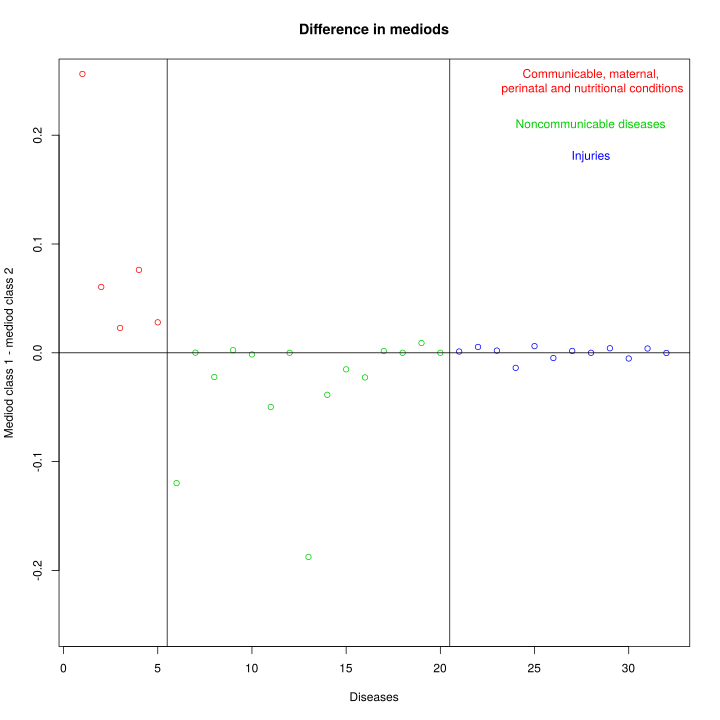
\includegraphics[width=\textwidth]{figures/difMediods.jpg}
	\caption{De verschillen van de gemiddelden}
	\label{fig:dm}
\end{figure}

\subsection{Principaalcomponentenanalyse}
\begin{figure}
	\centering
	\begin{subfigure}{\linewidth}
		\includegraphics[width = .5\linewidth]{figures/PC1vsPC2.png}
		\includegraphics[width = .5\linewidth]{figures/PC1vsPC3.png}
	\end{subfigure}
	\begin{subfigure}{\linewidth}
		\centering

	\end{subfigure}
	\begin{subfigure}{\linewidth}
		\centering
		\includegraphics[width = .5\linewidth]{figures/PC1vsPC4.png}
	\end{subfigure}
	\caption{De eerste principaalcomponent vergeleken met de andere drie belangrijkste principaalcomponenten}
	\label{fig:vglPC}
\end{figure}

 
\end{document}
